\chapter{Metodología} % Main chapter title
\label{Chapter2} % For referencing the chapter elsewhere, use \ref{Chapter1} 

\section{Metodología utilizada}

En el presente proyecto se ha utilizado la metología CRISP DM, pero sólo en las etapas iniciales que tienen que ver con el trabajo de los datos. En la imagen Figure~\ref{fig:crispdm} se pueden ver resaltadas las etapas cubiertas.

\begin{figure}[th]
\centering
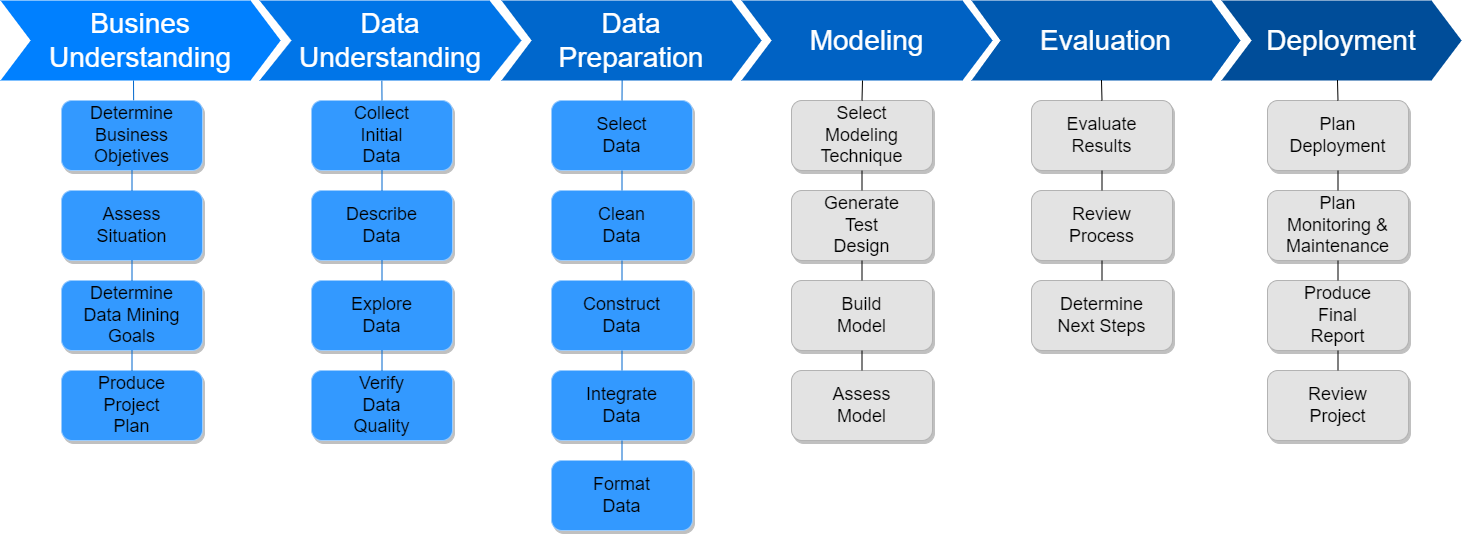
\includegraphics[width=1.2\textwidth]{Figures/modelo_crisp}
\decoRule
\caption[Metodolofía Crisp DM]{Secciones cubiertas en el proyecto}
\label{fig:crispdm}
\end{figure}

\section{Herramientas usadas}

Se han hecho uso de las siguientes herramientas:

\begin{itemize}
\item Base de datos MySql
\item Servicio RDS de AWS
\item R Studio
\item JetBrains DataGrip
\item Shiny
\end{itemize}

Se obtuvo un archivo CSV con toda la información de estudiantes, este archivo fue subido mediante DataGrip a una BD MySQL, previamente creada como un servicio RDS de AWS, con estos datos cargados se realizaron procesos mediante R para obtener información que posteriormente fueron registrados en otra base de datos y mostrados mediante una aplicación Shiny.

En la imagen Figure~\ref{fig:proceso} se puede ver el flujo del proceso en este trabajo de análisis.
\begin{figure}[th]
\centering
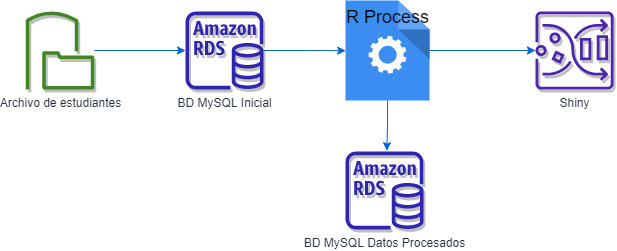
\includegraphics[width=1.1\textwidth]{Figures/proceso-archi}
\decoRule
\caption[Proceso de exploración de los datos]{Herramientas usadas}
\label{fig:proceso}
\end{figure}

\section{Trabajo con los datos}

Para el trabajo con R y MySQL se hizo uso de la bilbioteca RMySQL y DBI, el código para la conexión se encuentra en la sección \ref{codigo_conexionbd}.

\section{Uso de shiny}

...